\documentclass[12pt]{article}
\usepackage{graphicx}
\usepackage{amsmath}
\usepackage{float}

% Title and Author
\title{Lab 1: Introduction}
\author{Arnav Menon \\ School of Physics, Georgia Institute of Technology}
\date{January 21, 2025}

\begin{document}

\maketitle

\section*{Purpose}
The purpose of this lab is to gain familiarity with fundamental optical laboratory equipment and measurement techniques which will be utilized throughout the semester. Specifically, the experiment aims to measure the optical power of a helium-neon (HeNe) laser beam using a silicon photodiode detector, investigate the attenuation of laser light using neutral density filters, and analyze the AC fluctuations of an incandescent light source using an oscilloscope. This lab serves as an introduction to experimental methods that are used in optics and establishes foundational skills in data acquisition, analysis, and reporting.

\section*{Procedure}
\textbf{Measuring the laser power:}
\begin{enumerate}
    \item Mount the HeNe laser securely on the optical rail, ensuring its beam is aligned horizontally. Place the PDA55 optical detector about 40 cm from the laser output. Connect the detector to a digital multimeter (DMM) set to DC voltage mode. Record the voltage output from the detector and use the provided formula, \( P = 0.167 \cdot V \), to convert the voltage into optical power (in mW).
    \item Block the laser beam and measure the ambient light level reaching the detector. Subtract this value from the total measured power to isolate the laser power. Attach a lens tube to the detector to shield it from ambient light. Re-measure the voltage to confirm the reduced background light.
    \item Completely block all light from reaching the detector and measure its output voltage. This value represents the electronic offset, which should be noted.
\end{enumerate}
\textbf{Attenuating a laser beam using neutral density filters:}
\begin{enumerate}
    \item Place neutral density filters of varying optical density (OD = 0, 0.5, 1, 1.5, 2, 2.5, 3, 3.5, 6, 10) in the laser beam's path.
    \item Record the voltage readings for each OD value and calculate the transmitted power using the relation \( P_{transmitted} = P_{incident} \cdot 10^{-\text{OD}} \).
    \item Plot the transmitted power as a function of OD and fit the data to an appropriate exponential model.
\end{enumerate}
\textbf{AC fluctuations of incandescent light:}
\begin{enumerate}
    \item Replace the laser with an incandescent light source and connect the detector to an oscilloscope.
    \item Adjust the oscilloscope settings to measure the sinusoidal voltage signal. Record the peak-to-peak voltage, period, and frequency of the signal.
\end{enumerate}

\section*{Laser Power and Background Light}
To determine the optical power of the laser, the output beam was directed at the PDA55 detector connected to a digital multi-meter. A photograph of the experimental setup is shown in Fig. \ref{fig:setup}. The detector's voltage output, measured as 3 V, was converted to power using the conversion factor \(0.167 \, \text{mW/V}\), yielding a power of 0.501 mW. To measure the background light, the laser beam was blocked, and the detector voltage was measured as 0.020 V, corresponding to a power of 0.00334 mW.

Further reduction in background light was achieved by attaching a 3" lens tube, which led to readings of 0.008 V and 0.001336 mW. Finally, with all light sources blocked, the detector's electronic offset was recorded as 0.007 V and 0.001169 mW.

\begin{figure}
    \centering
    \includegraphics[width=\linewidth]{Screenshot 2025-01-21 at 1.44.50 PM.png}
    \caption{Setup with laser and photodetector connected to a digital multimeter.}
    \label{fig:setup}
\end{figure}

\section*{Attenuation from Neutral Density Filters}
To determine the effects of neutral density filters, various combinations were placed in the beam in front of the detector such that each data point had the OD values at OD = 0, 0.5, 1, 1.5, 2, 2.5, 3, 3.5, 6, 10. The power at the detector as a function of filter OD is shown in Fig. \ref{fig:exp-fit}, and on a logarithmic scale in Fig. \ref{fig:log-fit}. This dependence was fit to the equation \(y = y_0 +Ae^{-kx}\), and the best-fit values are \(y_0 = 2 \times 10^{-4}, A = 0.2061, k = 2.0156\).

\begin{figure} [H]
    \centering
    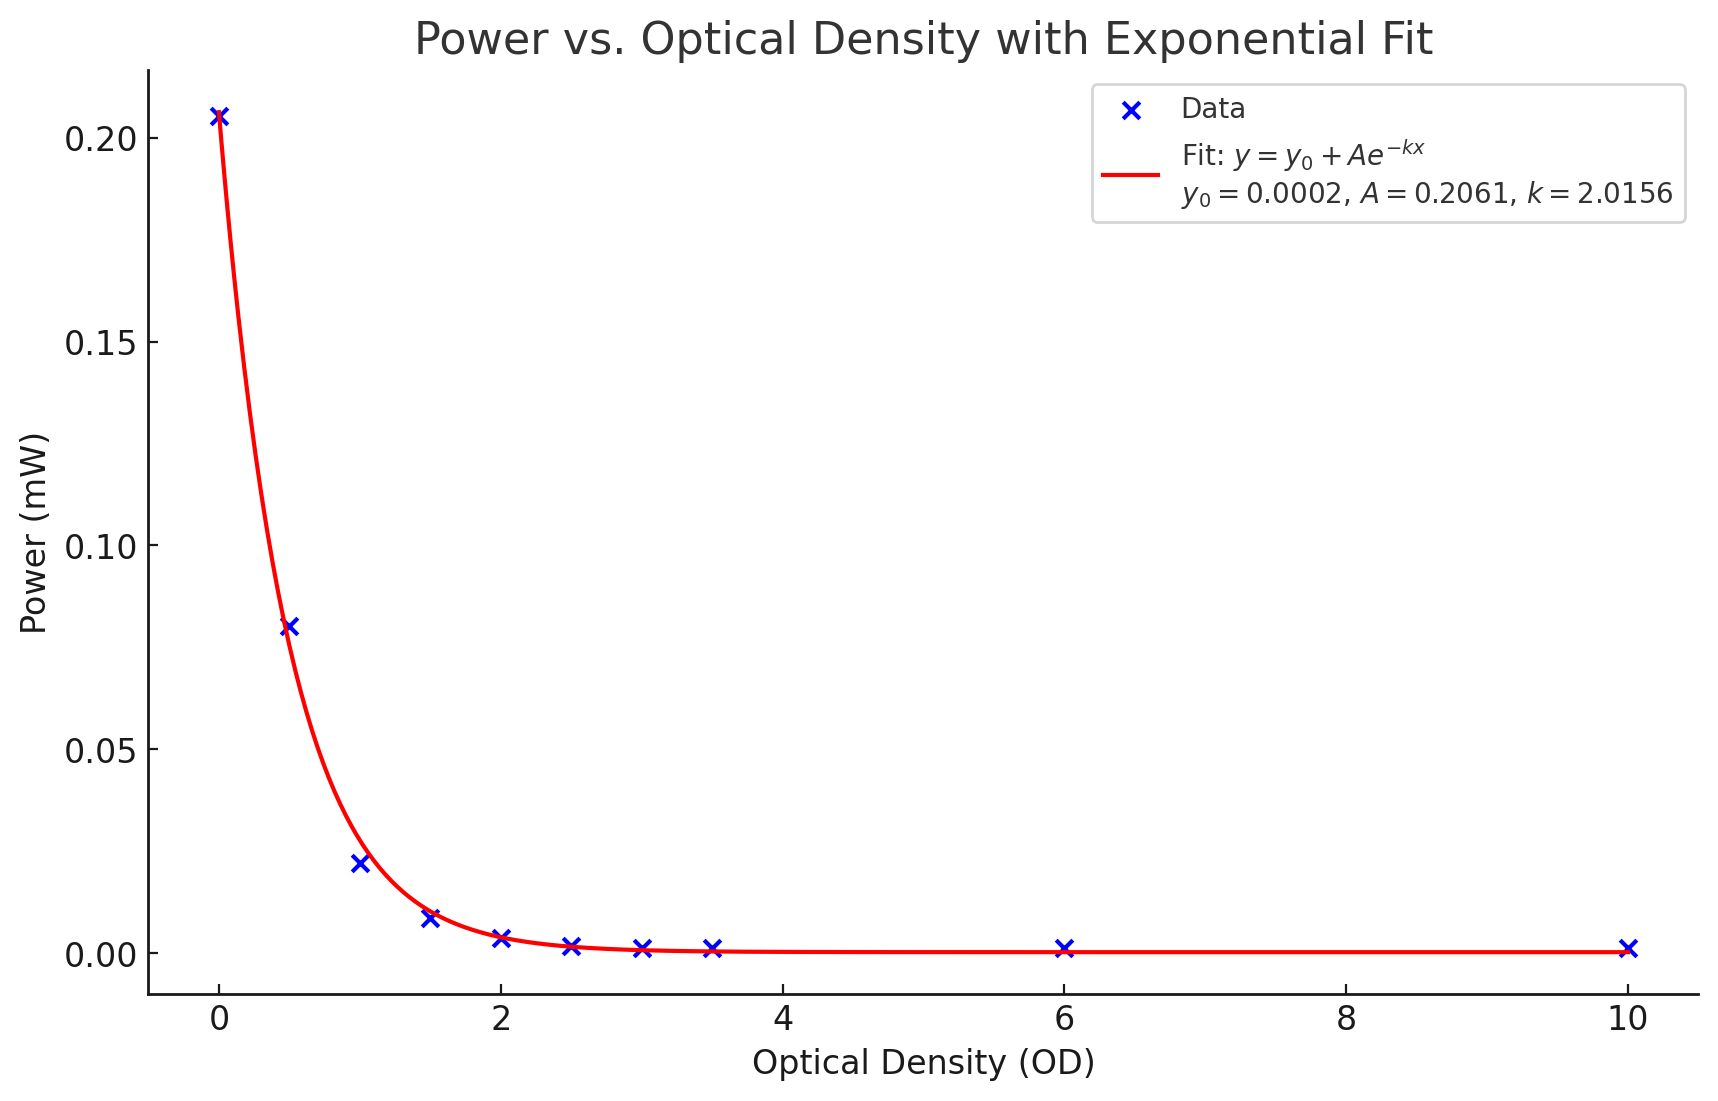
\includegraphics[width=0.8\linewidth]{Output from ChatGPT (1).png}
    \caption{Power vs. Optical Density fit. The blue points are the measured data and the red line is the exponential fit to the data.}
    \label{fig:exp-fit}
\end{figure}

\begin{figure} [H]
    \centering
    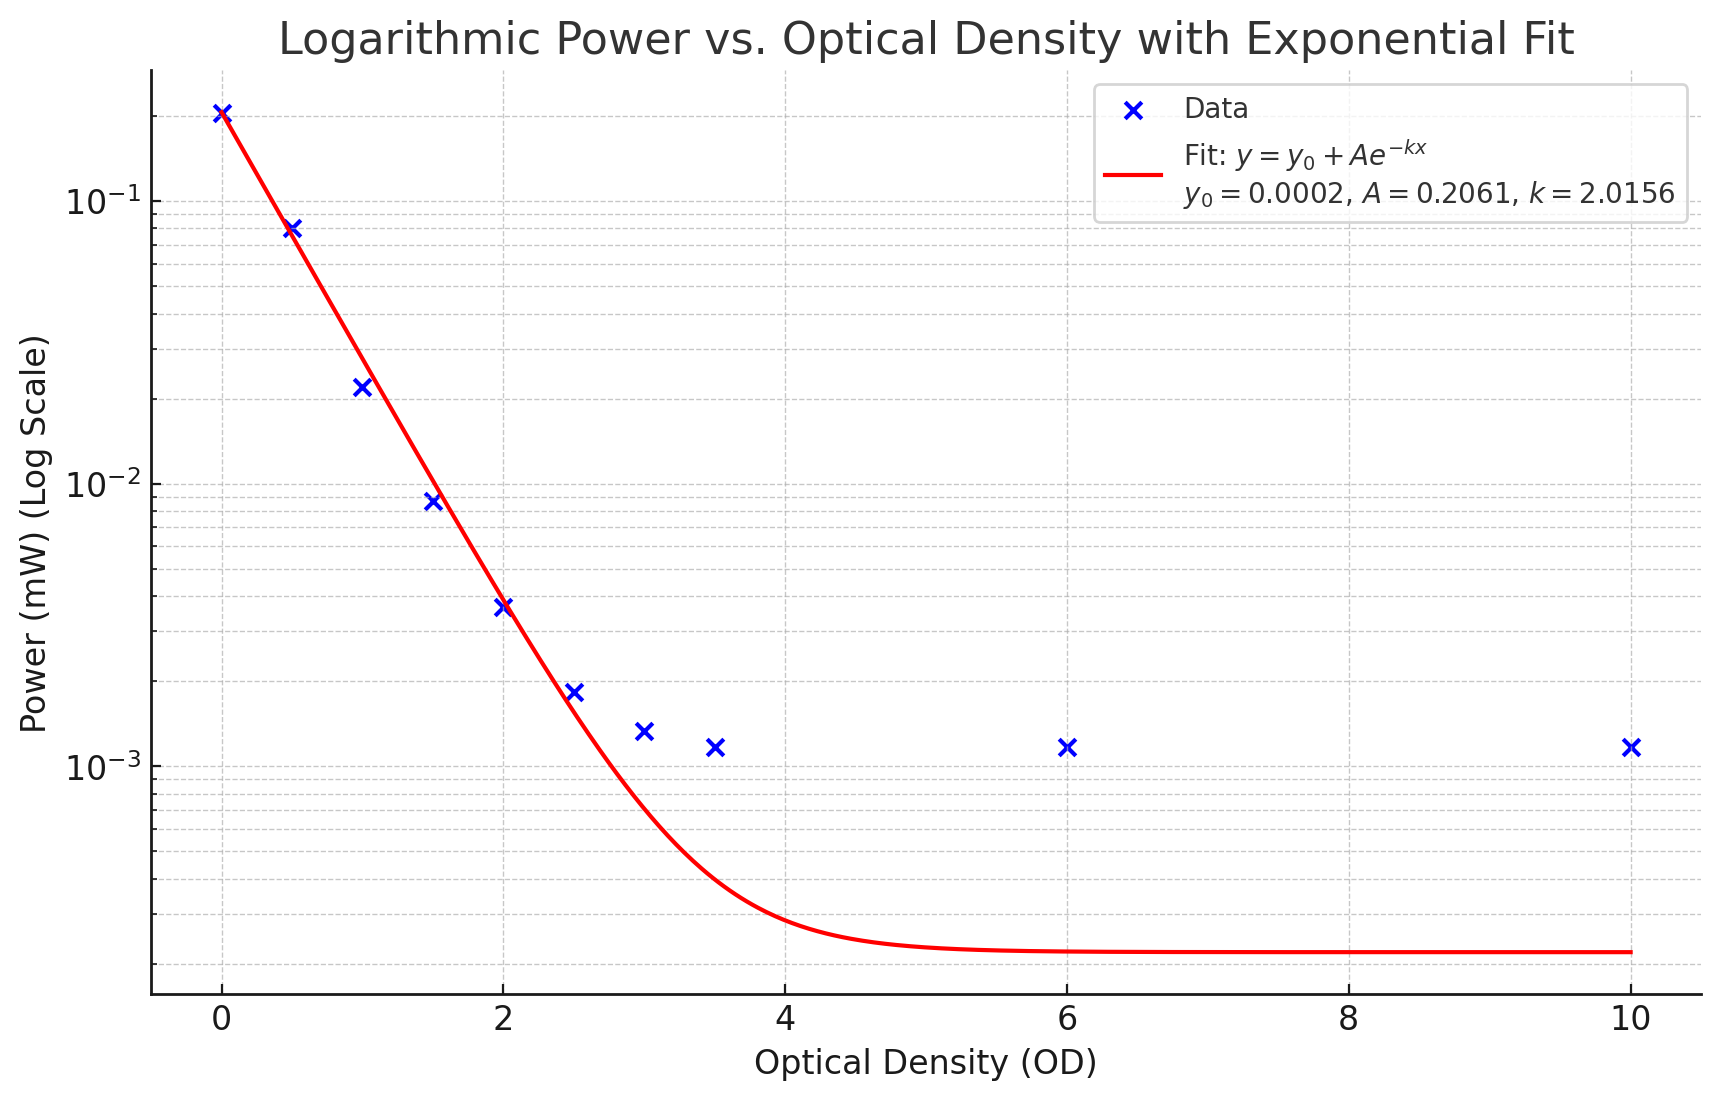
\includegraphics[width=0.8\linewidth]{Output from ChatGPT (2).png}
    \caption{Power vs. Optical Density fit. The blue points are the measured data and the red line is the exponential fit to the data, where the power axis is scaled logarithmically. A straight line fit can be seen until the optical density becomes too high and the value of \(y_0\) dominates.}
    \label{fig:log-fit}
\end{figure}

\section*{AC Fluctuations of Incandescent Light}
For this section, an incandescent light bulb was used to illuminate the detector instead of the laser. An oscilloscope was used to measure the voltage, setting the time scale to 10 ms per division. Photographs of the signal on the oscilloscope screen is shown in Fig. \ref{fig:oscilloscope}. and in Fig. \ref{fig:oscilloscope1}. The peak-to-peak voltage was measured to be 104 mV, and the average voltage can be found by multiplying this value by \(2 / \pi\), yielding 66.208 mV. The period of the signal was measured to be 8.4 ms, so the frequency of the signal is found to be 119.048 Hz.

\begin{figure} [H]
    \centering
    \includegraphics[width=\linewidth]{HEIC to PNG Conversion.png}
    \caption{Photograph of the oscilloscope reading from the incandescent light, showing the time difference between troughs.}
    \label{fig:oscilloscope}
\end{figure}

\begin{figure} [H]
    \centering
    \includegraphics[width=\linewidth]{HEIC to PNG Conversion (1).png}
    \caption{Photograph of the oscilloscope reading from the incandescent light, showing the amplitude of the signal.}
    \label{fig:oscilloscope1}
\end{figure}



\section*{Summary}
This lab provided a foundational understanding of optical laboratory equipment and techniques. The experiment successfully demonstrated the measurement of a helium-neon (HeNe) laser beam's optical power using a PDA55 photodiode detector. Through careful subtraction of background light and electronic offsets, accurate power readings were obtained. The attenuation of the laser beam was studied using neutral density filters, with results modeled by an exponential decay function. The fit parameters highlighted the relationship between optical density and transmitted power, as visualized on linear and logarithmic scales. Finally, the AC fluctuations of an incandescent light source were analyzed using an oscilloscope. Key parameters, including peak-to-peak voltage, average voltage, and signal frequency, were measured and linked to the light source's characteristics. Overall, this lab introduced essential skills in data acquisition, analysis, and reporting, forming the basis for more advanced optical experiments later in the semester.

\end{document}

